\section[ЛР №2. Модель обслуживания SaaS, ownCloud]{Лабораторная работа №2. \\
Модель обслуживания SaaS на примере развертывания облачного хранилища ownCloud}

\textbf{Цель работы:} ознакомиться с основными моделями представления облачных услуг (SaaS, PaaS, IaaS), развернуть собственное облачное хранилище, доступное пользователям в пределах локальной сети.

\subsection{Теоретические основы облачных вычислений}

Облачные вычисления (<<облака>>, Cloud computing) "--- модель предоставления вычислительных ресурсов, охватывающая все, от приложений и до центров обработки данных (ЦОД), через Интернет при условии оплаты за фактическое использование.

Одной из первых, кто стал внедрять услугу облачных вычислений стала компания Amazon, в то время (2002~г.) она еще являлась книжным Интернет-магазином, который впоследствии перерос, благодаря этим внедрениям, в одну из мощнейших технологических компаний.
Уже в 2006~г. был запущен проект под названием Computing Cloud (Amazon EC2)\footnote{\url{https://aws.amazon.com/ru/ec2/}}, после этого в 2009~г. компания Google представила Google Apps\footnote{\url{https://gsuite.google.com/}}.

После этих событий были сформированы общие понятия об облачных вычислениях, в частности выделены наиболее важные модели обслуживания и модели развертывания.

Облачные вычисления являются следующим шагом в эволюции архитектуры построения информационных систем.
Благодаря преимуществам данного подхода вполне очевидно, что многие информационные системы в ближайшее время переносятся или будут перенесены в облако.
Процесс уже идет полным ходом и его игнорирование или недооценка может привести к поражению в конкурентной борьбе на рынке.

Различают три основные модели обслуживания:
\begin{enumerate}
    \item программное обеспечение как услуга (Software as a Service, SaaS);
    \item платформа как услуга (Platform as a Service, PaaS);
    \item инфраструктура как услуга (Infrastructure as a Service, IaaS).
\end{enumerate}

Такие модели обслуживания как Container as a Service (CaaS) и Database as a Service (DaaS), являются по больше мере частными случаями IaaS и SaaS соответственно.

SaaS "--- модель, при которой не требуется приобретать, устанавливать, обновлять и поддерживать ПО, эту задачу берет на себя поставщик услуги.
Кроме того, осуществить регистрацию и использование облачных приложений можно немедленно, приложения и данные приложений доступны с любого устройства, подключенного к Интернету.
При поломке устройства данные не теряются, они хранятся в облаке, пользователю, как правило, доступны локальные настройки конфигурации приложения.

Примерами модели SaaS могут служить: почтовая служба Gmail, Dropbox, Google Docs, Microsoft Office 365.

PaaS "--- модель, при которой пользователю предоставляется возможность использования облачной инфраструктуры для размещения базового ПО.
В таком случае конфигурирование программного обеспечения целиком ложится на пользователя, предоставляется только платформа для развертывания ПО.

\clearpage

Примером модели PaaS является предоставление услуги развертывания собственного ПО в рамках облачной инфраструктуры, например Heroku, OpenShift.

IaaS "--- модель, при которой пользователю, доступно полное управление облаком в рамках операционной системы.
Потребитель обладает контролем над операционными системами, сетевыми сервисами.
Данная модель подходит задачам, для которых характерно быстрое изменение нагрузки.
Пользователю предоставляется виртуализированное окружение, как правило с <<чистой>> операционной системой, пригодной для развертывания любого приложения.

Примеры: Digital Ocean, Microsoft Azure, Google Compute Engine (GCE), Amazon Web Services (AWS).

\begin{figure}[ht]
    \centering
	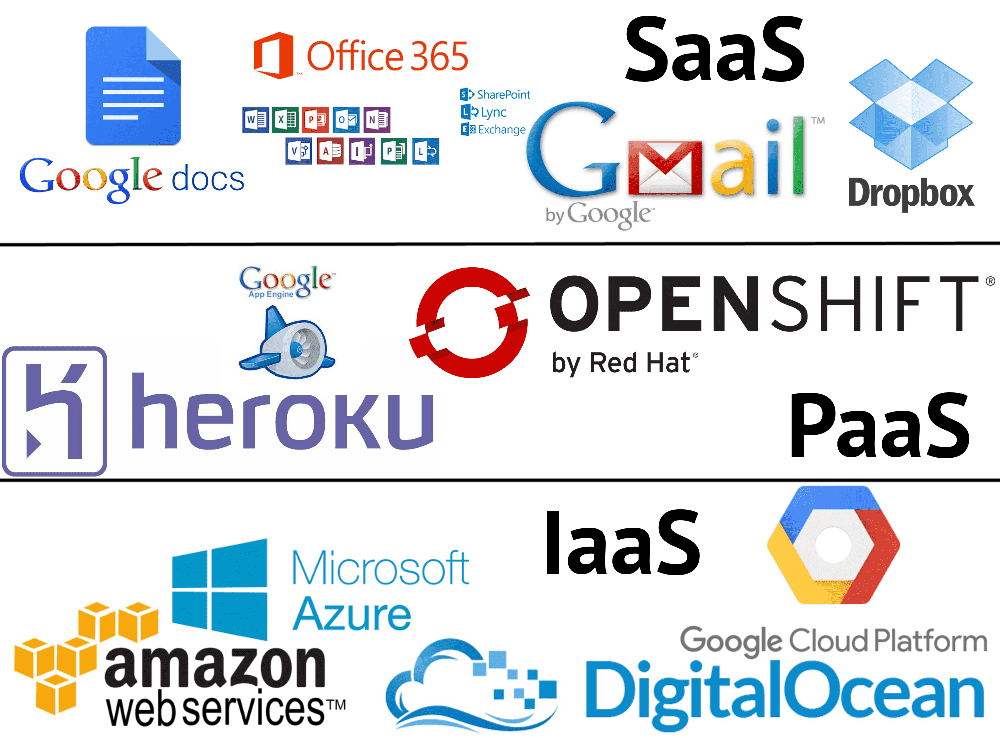
\includegraphics[width=\linewidth]{iaas-paas-saas}
	\caption{Представители различных моделей обслуживания}\label{pic:iaas-paas-saas}
\end{figure}

Модели развертывания облака можно разделить на четыре вида:
\begin{enumerate}
    \item частное облако (private cloud);
    \item публичное облако (public cloud);
    \item общественное облако (community cloud);
    \item гибридное облако (hybrid cloud).
\end{enumerate}

\clearpage

Частное облако предназначено для использования одной организацией, как правило оно находится в собственности самой организации.
Публичное облако предназначено для широкой публики, как правило находится в собственности сторонних организаций.
Общественное, как правило предназначено для сообщества или организации, а гибридное облако состоит из двух или более различных облачных инфраструктур.

\begin{figure}[ht]
    \centering
	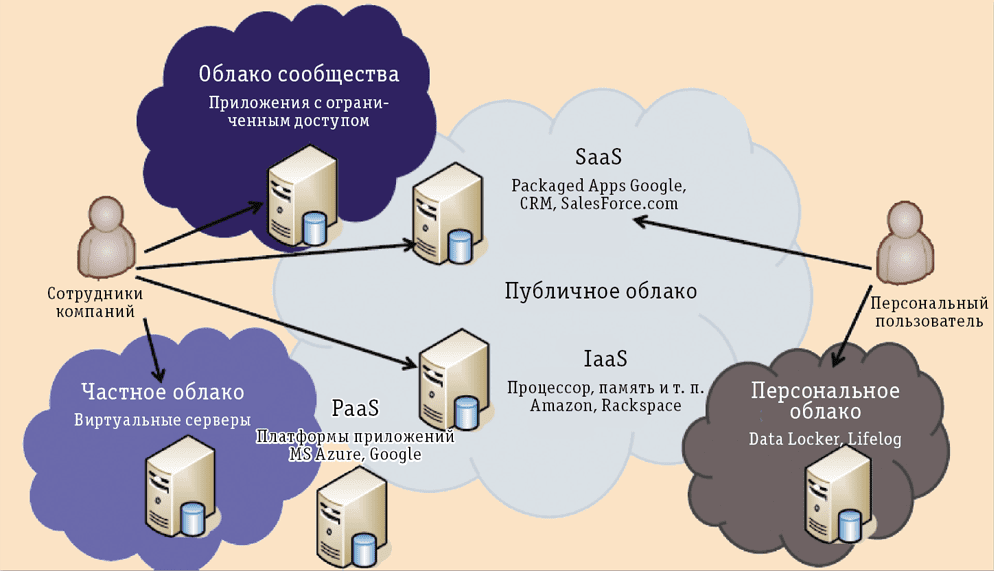
\includegraphics[width=\linewidth]{clouds}
	\caption{Различия между моделями развертывания облака}\label{pic:clouds}
\end{figure}

Основными преимуществами использования облачных технологий являются:
\begin{itemize}
    \item снижение расходов на закупку оборудования и построения центров обработки данных (ЦОД);
    \item удобство использования приложений с большого количества устройств, в том числе и мобильных;
    \item обеспечение надежности хранения данных, производительности приложений, за счет простоты использования ПО, мониторинга, балансировки нагрузки, миграции данных и~т.д.
\end{itemize}

ownCloud "--- свободное веб-приложение, предназначенное для синхронизации данных между сервером и клиентами, как правило данными являются документы и медиаконтент.
ownCloud является альтернативой таким облачным сервисам как Dropbox, Google Drive, Яндекс Диск, MEGA и др.
Отличие состоит в том, что приложение можно развернуть на собственном сервере как для домашнего использования, так и для использования в организациях.

Так как приложение распространяется бесплатно, имеет открытый исходный код\footnote{\url{https://github.com/owncloud/}} и периодически обрастает новыми функциями (планировщик задач, календарь, фотогалерея, просмотрщик документов, гибкая аутентификация пользователей и другие) проект обрел популярность как у пользователей, так и у Open-source разработчиков.

\subsection{Порядок выполнения работы}

Для выполнения лабораторной работы, в качестве сервера может использоваться виртуальная машина с ранее установленным (в ЛР№1) дистрибутивом Debian.
Виртуальная машина должна иметь доступ в сеть Интернет для скачивания нужных пакетов.

\begin{enumerate}
    \item Установить\footnote{Пример установки ownCloud Server представлен в прил.~\ref{pril:c}} ownCloud Server в виртуальную машину;
    \item На хост-машине или на другом компьютере сети скачать\footnote{\url{https://owncloud.org/install/}} и установить ownCloud Client;
    \item Подключить ownCloud Client к серверу во время первого запуска клиента, а также синхронизировать все данные с сервера\footnote{Пример настройки ownCloud Client представлен в прил.~\ref{pril:d}};
    \item Проверить работу синхронизации данных между клиентом и сервером (создать, удалить, переместить файл или каталог);
    \item Предоставить публичную ссылку на файл или каталог и проверить ее доступность в пределах локальной сети;
    \item Ознакомиться с дополнительными возможностями ownCloud.
\end{enumerate}

\subsection{Контрольные вопросы}
\begin{enumerate}
    \item Каковы основные преимущества использования облачных технологий?
    \item В чем состоит отличие SaaS от PaaS и IaaS?
    \item Какими преимуществами и недостатками обладает ownCloud по сравнению с Dropbox или другими облачными хранилищами?
    \item Почему одни организации предпочитают использовать в своей инфраструктуре частные облака, а другие "--- публичные?
\end{enumerate}

\clearpage
